
\chapter{Finding Minima of Neon Replacements}
\label{chap:Erstes Kapitel}
\section{Pair Potential Interaction}
\subsection{\ac{HF} equations}
We start with the pair potentials of Ne-Ne, Ne-Na and Na-Na to mimic the interaction of long distance van der Vaals + short distance repulsion forces. The pair potentials have been calculated using a \ac{HF} self consistent field cycle with \ac{MP2} by varying the atom distance. Now selfconsistently solving the equations:\\
\begin{align}
	\left[-\frac{\hbar^2}{2m}\vec{\nabla}^2-\frac{Ze^2}{4\pi\varepsilon_0}-\frac{e^2}{4\varepsilon_0}\sum_{\nu,\sigma}^{(\mu\sigma)\neq(\nu\sigma)}\iiint_{\mathbb{R}^3}\frac{\varphi_{\nu\sigma'}(\tilde{\vec{r}})}{\|\vec{r}-\tilde{\vec{r}}\|}\mathrm{d}^3\tilde{\vec{r}}-\hat{A}_{\mu\sigma}(\vec{r})\right]\varphi_{\mu\sigma}(\vec{r})=\varepsilon_{\mu\sigma}\varphi_{\mu\sigma}(\vec{r}),
\end{align}
with $\hat{A}_{\mu\sigma}$ being the exchange correlation term leads to the eigenenergies $\varepsilon_{\mu\sigma}$. Since \ac{HF} 
minimizes a slater determinant, the energies correspond to the factors of the slater product state, meaning the systems energy is the sum of the energy of the single electrons. From that, to get the actual energy of the whole system, one needs to remove inter-electron repulsion and exchange correlation from the sum of all eigenenergies $\varepsilon_{\mu\sigma}$:
\begin{align}
	E_{HF}^0 = \sum_{\mu,\sigma}\varepsilon_{\mu\sigma}-\frac{1}{2}\sum_{\substack{\mu,\nu\\\sigma,\sigma'}}^{(\mu\sigma\neq\nu\sigma)}\left[C_{\mu\sigma}^{\nu\sigma'}-A_{\mu\sigma}^{\nu\sigma}\delta_{\sigma\sigma'}\right]
\end{align}
with $C_{\mu\sigma}^{\nu\sigma'},A_{\mu\sigma}^{\nu\sigma}$ being defined as:
\begin{align}
	C_{\mu \sigma}^{v \sigma^{\prime}}&=\frac{e^2}{4 \pi \varepsilon_0} \iint  \frac{\left|\varphi_{\mu \sigma}(r)\right|^2\left|\varphi_{v \sigma^{\prime}}\left(r^{\prime}\right)\right|^2}{\left|r-r^{\prime}\right|}\mathrm{~d}^3 r \mathrm{~d}^3 r^{\prime},
	\\
	A_{\mu \sigma}^{v \sigma}&=\frac{e^2}{4 \pi \varepsilon_0} \iint \frac{\varphi_{\mu \sigma}^*(r) \varphi_{v \sigma}^*\left(r^{\prime}\right) \varphi_{\mu \sigma}\left(r^{\prime}\right) \varphi_{v \sigma}(r)}{\left|r-r^{\prime}\right|} \mathrm{~d}^3 r \mathrm{~d}^3 r^{\prime}.
\end{align}
Since solving the \ac{HF} equations in real space is too costly one restricts the variations to coefficients of a superposition of fixed basis vectors. These lead to the Roothaan-Hall equations, which are a discrete Matrix representation of the \ac{HF} equations:
\begin{align}
	\mathbf{F C}=\mathbf{S C} \epsilon,
	\label{eq:roothaan}
\end{align} 

with $\epsilon$ being a diagonal matrix of single particle energies on the diagonal, $\mathbf{S}$ the basis overlap matrix, $\mathbf{C}$ the coefficient matrix and finally $\mathbf{F}$ the Fock operator.
\subsection{Møller-Plesset Perturbation}
Møller-Plesset Perturbation theory extends the idea of \ac{HF}. We consider the actual true Hamiltonian  $\hat{H}$ in the same basis as \ref{eq:roothaan} and define the difference to the Fock operator to be a relatively small perturbation:
\begin{align}
	\hat{H}= \hat{F} + \underbrace{\left(\hat{H}-\hat{F}\right)}_{\hat{V}_{pert}}.
\end{align}
Now the $0$-th order terms of the perturbation are
\begin{align}
	E^{(1)}&=\bra{\Psi_{HF}}\left(\hat{H}-\hat{F}\right)\ket{\Psi_{HF}}=\\
	&=-\frac{1}{2}\sum_{\mu\nu}\left[\bra{\varphi_{\mu}\varphi_{\nu}}\hat{V}^{(2)}(\hat{\vec{r}}_\mu,\hat{\vec{r}}_\nu)\ket{\varphi_{\mu}\varphi_{\nu}}-\bra{\varphi_{\mu}\varphi_{\nu}}\hat{V}^{(2)}(\hat{\vec{r}}_\mu,\hat{\vec{r}}_\nu)\ket{\varphi_{\nu}\varphi_{\mu}}\right].
\end{align} 
which is exactly the mean-field and the exchange correlation term in the \ac{HF} Ansatz. To go beyond \ac{HF} we need to consider \ac{MP2}:
\begin{align}
	E^{(2)}=\sum_{\substack{N<a<b \\ \mu<\nu \leq N}} \frac{\left|\bra{\psi_0}\hat{V}^{(2)}(\hat{\vec{r}}_\mu,\hat{\vec{r}}_\nu)\ket{\psi_{\mu\nu}^{a b}}\right|^ 2}{\left(\varepsilon_a+\varepsilon_b\right)-\left(\varepsilon_\mu+\varepsilon_\nu\right)} .
\end{align} where $\ket{\psi_{\mu\nu}^{a b}}$ is an excited Slater determinant, where single orbitals $\mu, \nu$ are removed and replaced by single orbitals $a,b$ in the slater determinant. $\varepsilon_i$ are eigenvalues of the slater single particle factors of the \ac{HF} problem.
\subsection{\ac{BSSE}}
Now the the superpositions of a fixed basis leads to the \ac{BSSE}. These errors are being corrected for by using 'ghost calculations', essentially the same calculation with one atom being removed (i.e. the extended two atom centered basis stays the same). This means the basis will have access to the second electron states, but the nucleus and additional electrons are not accounted for. These 'ghost energies' will then subsequently be removed from the \ac{HF}
approximation to correct for the \ac{BSSE}.
This is know as the counterpoise‐corrected interaction energy formula or Boys–Bernardi method: %TODO citation %TODO fix formula
\begin{align}
	E_{\text {int}}^{\text {CP}}(R)=E_{A B}(R)-E_A^{\text {ghost}}(R)-E_B^{\text {ghost}}(R).
\end{align}
\subsection{Interpolation}

\begin{figure}[h!]
	\centering
	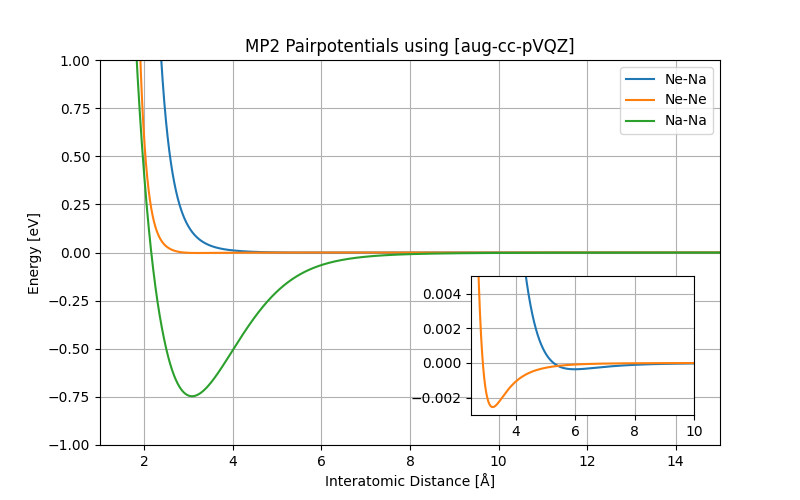
\includegraphics[scale = 0.7]{Inhalt/Bilder/pairpotential.png}
	\caption{Plots of interpolations of pair potentials of Ne-Ne, Na-Na, Ne-Na calculated with Moeller Plesset 2 perturabtion theory.}
	\label{fig:pairpotential}
\end{figure}
%TODO Noltig source
-explain exact interpolation\\
-paper citation where brute force plot shows up as well\\
-which basisi is being used in the roothaan equations \\
-explain setup of calculation with ball being carved out\\
-maybe here explain the nearest neighbours\\
lammps gets linear interpolation\\
-since plot is in priniple linearly interpolated this is the exact pair interactins that lammps will read
\section{Geometric LAMMPS Setup}
%%%%%%%%%%%%%%%%%%%%%%%%%%%%%%%%%%%%%TODO%%%%%%%%%%%%%%%%%%%%%%%%%%%
The simulation models a finite spherical cluster of atoms extracted from a bulk face-centered cubic lattice. To balance computational efficiency with physical realism, the system is partitioned into two concentric spherical regions defined in units of the lattice constant. The inner spherical region, with radius $n_{inner}$ contains atoms that are free to move and evolve dynamically. This region represents the core of the cluster where physical process and in this case the energy minimization via a relaxation calculation of \ac{LAMMPS} takes place.

Sourrounding this core is an immobilized shell with thickness $n_{outer}$
Atoms within this outer shell are constrained by setting their forces to zero, effectively fixing them in space. This fixed shell act as a rigid boundary that suppresses surface effects and mimics the presence of a an extended bulk lattice, thereby reducing finite size artifact in the dynamics of the inner region.

Consequently the total cluster is confined within a spherical domain of radius $R_{tot}=(n_{inner}+n_{outer})\cdot a$ with $a$ being the lattice constant of the pure neon \ac{fcc} lattice. 

Technically the simulation is defined as a cubic volume large enough to contain the entire spherical cluster, with half-length at least $R_{tot}$.
For the relaxation mechanics atomic positions are set according to \ref{fig:lammpssetup} on a perfect \ac{fcc} lattice no matter their role (sodium defect, fixed neon, dynamic neon) as long as they are inside the cutoff radius $R_{tot}$.
%TODO is it really ? check, cite
This approach is commonly employed in molecular dynamics studies to simulate nanoparticles or finite clusters embedded in bulk-like surroundings.
%%%%%%%%%%%%%%%%%%%%%%%%%%%%%%%%%%%TODO%%%%%%%%%%%%%%%%%%%%%%%%%%%%%%%%%%%
\begin{figure}[h!]
	\centering
	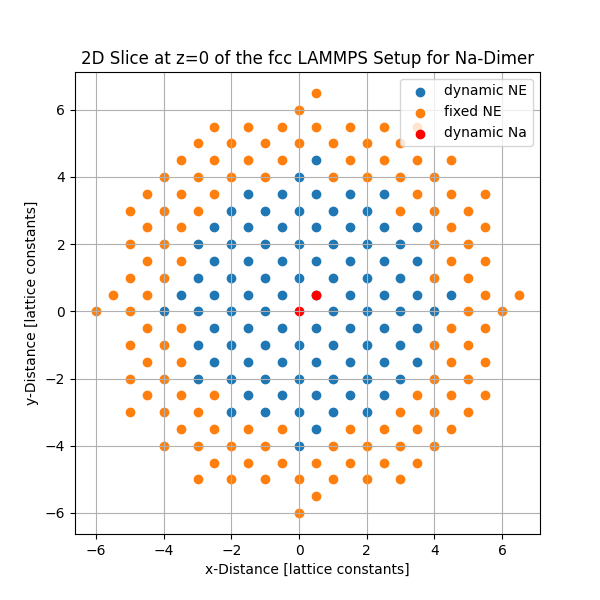
\includegraphics[scale=0.45]{Inhalt/Bilder/lammps_dimer_setup.png}
	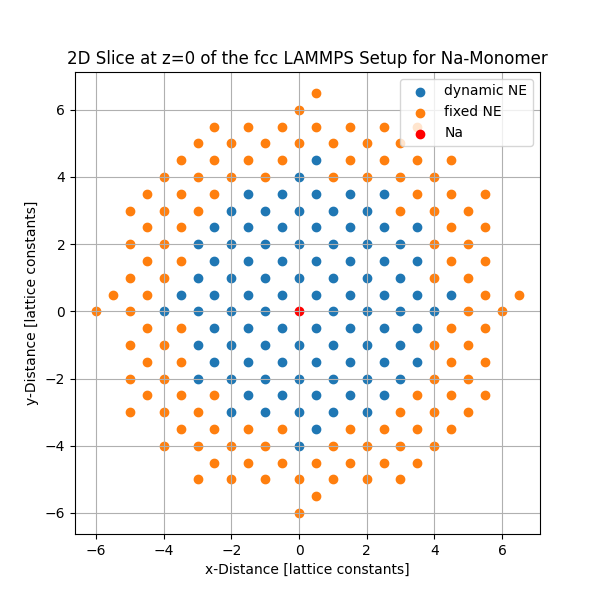
\includegraphics[scale=0.45]{Inhalt/Bilder/lammps_mono_setup.png}
	\caption{Initial setup for the \ac{LAMMPS} relaxation. Only the inner blue sphere is allowed to relax, forces on the orange atom positions are overridden to 0.}
	\label{fig:lammpssetup}
\end{figure}\\%TODO split figure into subfigures with exra captions
The centered red dots in \ref{fig:lammpssetup} represent sodium atoms. They represent the initial pre-relaxation positions of sodium inside the dynamic inner sphere. These initial positions are the same for every relaxation step of the simulated annealing. Note that the minimum energy of the pair-potential in \ref{fig:pairpotential} is roughly at $3\text{.}1\si{\angstrom}$ which is the nearest neighbor distance in the neon \ac{fcc} lattice. With $a = 4\text{.}4637\si{\angstrom}$: 
%TODO fix unit separator to a dot, onyl comma works for now
\begin{gather}
	\vec{a}_1=\begin{bmatrix}a\\0\end{bmatrix} \qquad \vec{a}_2=\begin{bmatrix}0\\a\end{bmatrix}\\
	\Rightarrow \|\frac{1}{2}\left(\vec{a}_1+\vec{a}_2\right)\|=\frac{1}{\sqrt{2}}\cdot a = 3\text{.}1563\si{\angstrom}.
\end{gather}  We therefore put the second sodium atom in the dimer calculations at the nearest neighbor lattice site. 
\section{Sodium Monomer}
Now the annealing was done as described in the chapters before for a single sodium atom at the center. Since the known energetically minimal configurations for every $S$ and it's corresponding energy was known due to a brute force calculation, this calculation serves as a benchmark for the annealing algorithm. The brute force minimal energies for the vacancies are shown in \ref{fig:simulatedannealingsodium} on the right axis. The left axis shows the relative counts (with respec to the total counts) of one annealing sweep consisting of itself 1000 random removals of neon atoms from the state vector. This annealed approach quickly converges to a statistical distribution shown in the same figure \ref{fig:simulatedannealingsodium} on the left $y$-axis. The pattern surfaces quickly after about 50 sweeps, the total amount of sweeps for the plot were 736. The true local minima at $S=10$ and $S=13$ could be picked up upon quite sharply. At $S=8$ the annealing algorithm seems to pick up on the notch, that is not quite an actual minima but could look like a local minima if approached from many directions in the high dimensional phase space.\\  
-Not feasible to brute force dimer with 3rd nearest neighbors\\
-explain nearest neighbors\\
-even with full 48 cubic point symmetry of the host of the defect which no structure can exceed ...\\ 
-explain confirmation of algorithm with brute force for mono sodium\\
-explain how plot is created with sweeps\\
-more complicated symmetries\\
-compare figures\\
-calculation for dimer\\
-discuss noteworthy structure (e.g. inner shell carved out)\\
-citation of paper that has the same plot
Now first by brute force search we know the minima for a single sodium atom.

%\begin{figure}[h!]
%	\centering
%	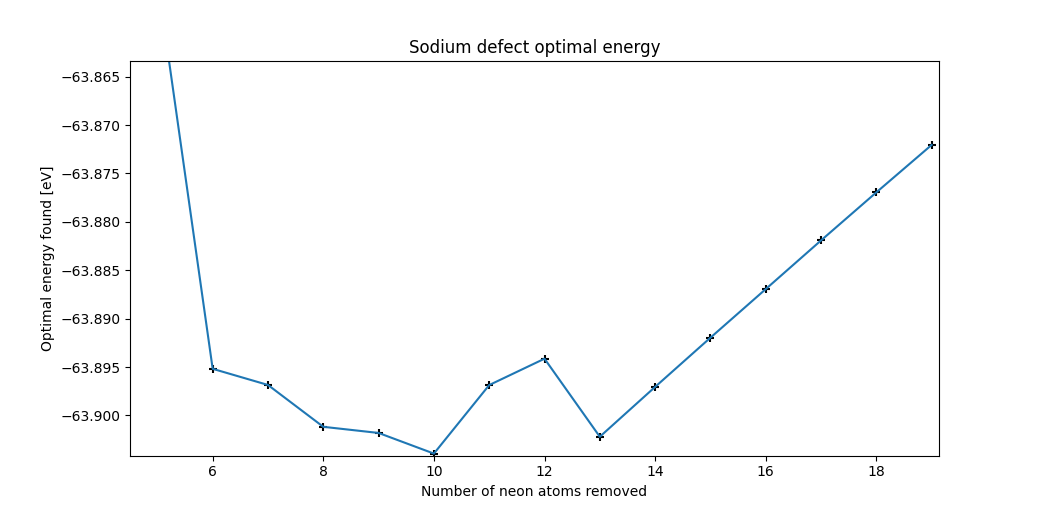
\includegraphics[scale=0.5]{./Inhalt/Bilder/optimal_defect_brute_force.png}
%	\caption{Brute force for single sodium atom}
%	\label{fig:bruteforcesodium}
%\end{figure}

\begin{figure}[h!]
	\centering
	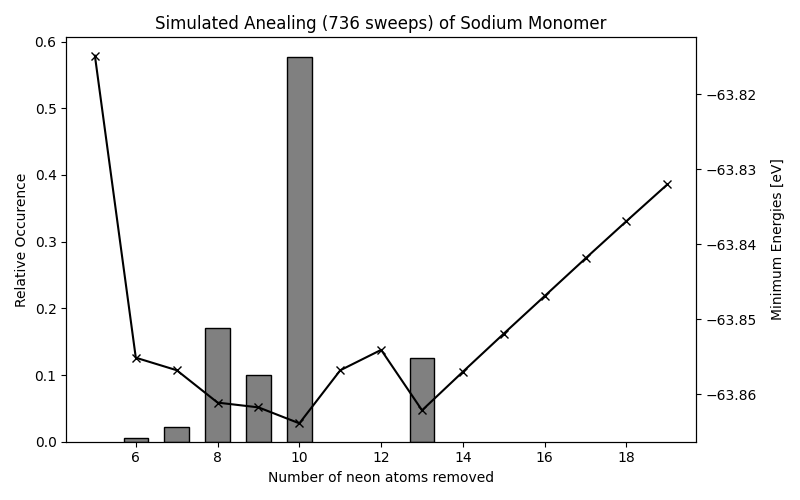
\includegraphics[scale=0.5]{./Inhalt/Bilder/optimal_defect_simulated_annealing.png}
	\caption{Simulated Annealing for single sodium atom inserted, compared to a brute force minima search for a fixed number of removed atoms S.}
	\label{fig:simulatedannealingsodium}
\end{figure}  

Since \ref{fig:simulatedannealingsodium} shows the simulated annealing algorithm accurately picks up on the location of the minima (albeit with no quantitative measure and misleading local minima being blown out of proportion (See $S=8$)) we try the same approach for the sodium dimer. Here the energetically optimal $S$ replacement will exceed the number of available sites as in the monomer calculation (i.e. up to second nearest neighbor). The sweeps and their random removal of neon atoms now act upon an extended state vector containing every lattice site up to the 3rd nearest neighbor. This is also the very reason a brute force approach is unfeasable, since the volume of phasespace to be explored grows quickly. This is the reason the statistical approach was chosen in the first place. 


-brute force lexiciraphically sorting algorithm here

\section{Sodium Dimer}
-in setup exxplain that dimer binding position is roughly first nearest neighbour of  ne lattice\\
-3rd nearest neighbors, why ? because minima is more the 2 shells
-rough estimate of time used by brute forcing\\
-even with full cubic symmetry this is too long (divide b 64)\\
-maybe think about symmetry\\
-same graphics as for the monomer case\\
-heuristically take the maxima of these plots \\
-give structures\\
-discuss structures (inner shell carved out)\\

\begin{figure}[h!]
	\centering
	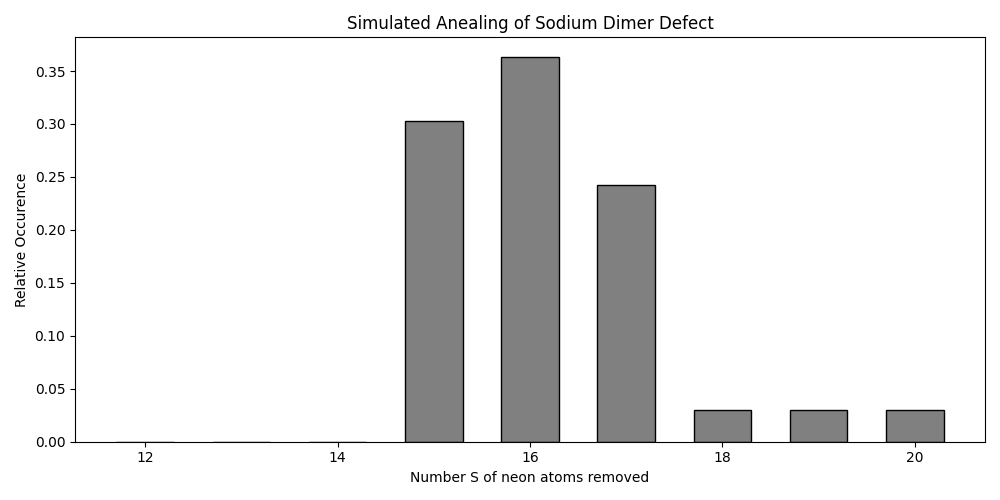
\includegraphics[scale = 0.5]{Inhalt/Bilder/optimaldimer.png}
	\caption{Simulated annealing results and their relative occurrence after x sweeps}
	\label{fig:simulatedannealingsodiumdimer}
\end{figure}

\chapter{DFT optical spectra results}
\label{chap:Zweites Kapitel}
%
Zweites Kapitel
%
%
\chapter{Conclusion}
Unfortunately no confidence or error can be estimated since the approach was purley heuristcal. Optical spectrum does not depend much on replacements and precise structure.



